\chapter{Future Work}

Future Features that could be added:

\section{Configuration file generation}
    yml config generation.
    These files are needed by the GPRM to determine aliases in GPIR code, libraries used,
    number of threads/nodes. There is enough information at compilation time to generate these,
    and they are currently generated manually. 


\section{Language Features}
    Other C++ language features, C++11 lambdas may be useful,
    while-loops, and possibly some STL support e.g. ability to use STD vector instead of pointers.

\section{Compiler Optimisations}

    There are a few optimisations that can be performed by the compiler to reduce the work needed to be 
    performed by the GPRM at runtime.

\subsection{Binary Expression Reduction}
Given the following GPC code:    

\lstinputlisting[style=myGPC]{code_samples/binaryOp.gpc}

In line 8, the expression within the m2 method call results in part of the Abstract Syntax Tree
which is represented as a Binary Expression Tree when parsed. Binary operators are contained in
the inner nodes with literal values and variables at the leaf nodes. 

\begin{center}
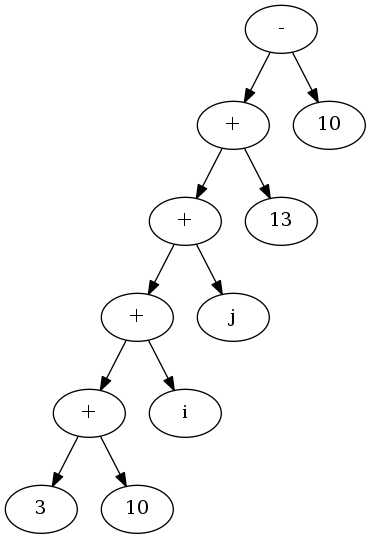
\includegraphics[scale=0.4]{graphs/evalTree.png}
\end{center}

During the evaluation stage of compilation the tree is evaluated through
postorder traversal. Once two leaf nodes are found the binary operation in the parent node
is attempted to be applied to the two leaf nodes. If both leaf nodes are values which
can be calculated at compile time the expression is evaluated, the two leaf nodes
are removed and the parent node is replaced with the calculated value. If one or
more leaf nodes are values which can only be known at runtime then the expression is
not evaluated and the tree doesn't change. 

The tree above once evaluated transforms into the following tree: 

\begin{center}
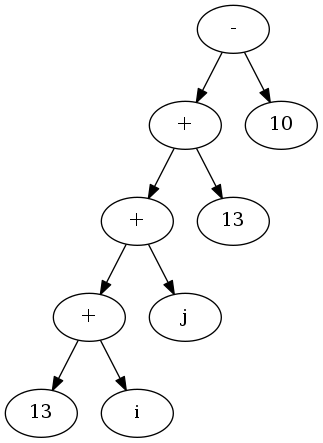
\includegraphics[scale=0.4]{graphs/fullyEvalTree.png}
\end{center}

We can see this reduction in the generated GPIR code:

\lstinputlisting[style=myGPIR]{code_samples/binaryOp.td}

The downsides of this method is that once
a value that can't be worked out at compile time is met, it is not possible
to evaluate expressions any value further up the tree. In the given example
it is clear that it is possible to evaluate the expression further.

One way to improve the evaluator would be to transform the tree before evaluating it.
Using the axioms of the binary operations in the tree (e.g. addition being associative)
and the type of values in the leaf nodes,. it should be possible to rearrange the nodes in the 
tree to create a new tree which represents an expression equivalent to the expression
represented by the starting tree.

The specific details of how the tree transformations work and implementation into the compiler is 
left as future work.

In this example, one "optimal" transformation of the tree would result in the following tree:

\begin{center}
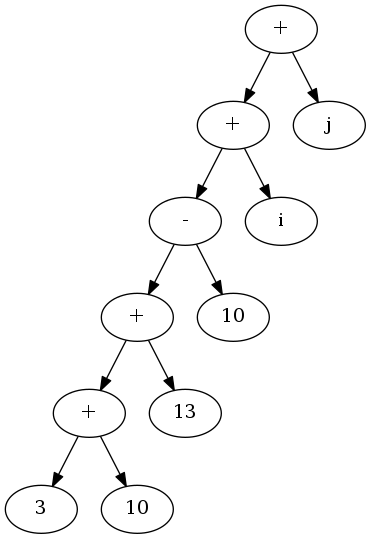
\includegraphics[scale=0.4]{graphs/optimalEvalTree.png}
\end{center}

The evaluator would then reduce this tree down to the following tree:

\begin{center}
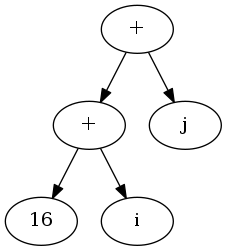
\includegraphics[scale=0.4]{graphs/optimalFullyEvalTree.png}
\end{center}

This generates much simpiler GPIR code:
\lstinputlisting[style=myGPIR]{code_samples/binaryOpImproved.td} 


\subsection{Pure Function Reduction}

When a function is pure (i.e. it contains no method calls
on kernel objects, and all arguments given to it when it is called can be evaluated at 
compile time) the function call should be able to be evaluated down to a single constant value.

The following GPC code is used as an example:

\lstinputlisting[style=myGPC]{code_samples/pureFun.gpc}

The function "f" does not call any methods on kernel objects, and has no arguments.
Every time "f" is called it returns the integer value "2". Therefore wherever f is called can
be replaced with the integer value "2". However the compiler generates the following GPIR code
for this example:

\lstinputlisting[style=myGPIR]{code_samples/pureFun.td}

When "f" is called its value is stored in a register. This is currently how function calls
store their return value when evaluated. An improvement to function evaluation to support
reduction of "pure functions" would result in generating this simpler GPIR code:

\lstinputlisting[style=myGPIR]{code_samples/pureFunImproved.td}
